\documentclass[14pt]{extbook}
\usepackage{multicol, enumerate, enumitem, hyperref, color, soul, setspace, parskip, fancyhdr} %General Packages
\usepackage{amssymb, amsthm, amsmath, latexsym, units, mathtools} %Math Packages
\everymath{\displaystyle} %All math in Display Style
% Packages with additional options
\usepackage[headsep=0.5cm,headheight=12pt, left=1 in,right= 1 in,top= 1 in,bottom= 1 in]{geometry}
\usepackage[usenames,dvipsnames]{xcolor}
\usepackage{dashrule}  % Package to use the command below to create lines between items
\newcommand{\litem}[1]{\item#1\hspace*{-1cm}\rule{\textwidth}{0.4pt}}
\pagestyle{fancy}
\lhead{Progress Quiz 7}
\chead{}
\rhead{Version C}
\lfoot{4173-5738}
\cfoot{}
\rfoot{Spring 2021}
\begin{document}

\begin{enumerate}
\litem{
Determine the horizontal and/or oblique asymptotes in the rational function below.\[ f(x) = \frac{5x^{2} +13 x -6}{20x^{3} -13 x^{2} -23 x + 10} \]\begin{enumerate}[label=\Alph*.]
\item \( \text{Horizontal Asymptote at } y = -3.000 \)
\item \( \text{Horizontal Asymptote of } y = 0.250 \text{ and Oblique Asymptote of } y = 4x -13 \)
\item \( \text{Oblique Asymptote of } y = 4x -13. \)
\item \( \text{Horizontal Asymptote of } y = 0 \)
\item \( \text{Horizontal Asymptote of } y = 0.250  \)

\end{enumerate} }
\litem{
Determine the vertical asymptotes and holes in the rational function below.\[ f(x) = \frac{16x^{3} +40 x^{2} +x -30}{8x^{2} +6 x -9} \]\begin{enumerate}[label=\Alph*.]
\item \( \text{Vertical Asymptotes of } x = -1.5 \text{ and } x = 0.75 \text{ with no holes.} \)
\item \( \text{Vertical Asymptote of } x = 2.0 \text{ and hole at } x = 0.75 \)
\item \( \text{Holes at } x = -1.5 \text{ and } x = 0.75 \text{ with no vertical asymptotes.} \)
\item \( \text{Vertical Asymptotes of } x = -1.5 \text{ and } x = -1.25 \text{ with a hole at } x = 0.75 \)
\item \( \text{Vertical Asymptote of } x = -1.5 \text{ and hole at } x = 0.75 \)

\end{enumerate} }
\litem{
Determine the vertical asymptotes and holes in the rational function below.\[ f(x) = \frac{8x^{3} +22 x^{2} -x -15}{8x^{2} -18 x + 9} \]\begin{enumerate}[label=\Alph*.]
\item \( \text{Vertical Asymptote of } x = 1.5 \text{ and hole at } x = 0.75 \)
\item \( \text{Vertical Asymptotes of } x = 1.5 \text{ and } x = 0.75 \text{ with no holes.} \)
\item \( \text{Vertical Asymptote of } x = 1.0 \text{ and hole at } x = 0.75 \)
\item \( \text{Holes at } x = 1.5 \text{ and } x = 0.75 \text{ with no vertical asymptotes.} \)
\item \( \text{Vertical Asymptotes of } x = 1.5 \text{ and } x = -2.5 \text{ with a hole at } x = 0.75 \)

\end{enumerate} }
\litem{
Determine the vertical asymptotes and holes in the rational function below.\[ f(x) = \frac{6x^{3} -5 x^{2} -61 x -60}{12x^{2} +11 x -15} \]\begin{enumerate}[label=\Alph*.]
\item \( \text{Vertical Asymptotes of } x = 0.75 \text{ and } x = -1.5 \text{ with a hole at } x = -1.667 \)
\item \( \text{Vertical Asymptote of } x = 0.75 \text{ and hole at } x = -1.667 \)
\item \( \text{Holes at } x = 0.75 \text{ and } x = -1.667 \text{ with no vertical asymptotes.} \)
\item \( \text{Vertical Asymptotes of } x = 0.75 \text{ and } x = -1.667 \text{ with no holes.} \)
\item \( \text{Vertical Asymptote of } x = 0.5 \text{ and hole at } x = -1.667 \)

\end{enumerate} }
\litem{
Determine the horizontal and/or oblique asymptotes in the rational function below.\[ f(x) = \frac{16x^{3} -16 x^{2} -81 x -45}{4x^{2} -13 x -12} \]\begin{enumerate}[label=\Alph*.]
\item \( \text{Horizontal Asymptote of } y = 4.0  \)
\item \( \text{Horizontal Asymptote of } y = 4.0 \text{ and Oblique Asymptote of } y = 4x + 9 \)
\item \( \text{Horizontal Asymptote at } y = 4.0 \)
\item \( \text{Horizontal Asymptote of } y = 4.0 \text{ and Oblique Asymptote of } y = 4x + 9 \)
\item \( \text{Oblique Asymptote of } y = 4x + 9. \)

\end{enumerate} }
\litem{
Determine the horizontal and/or oblique asymptotes in the rational function below.\[ f(x) = \frac{6x^{3} +41 x^{2} +89 x + 60}{-4x^{3} -28 x^{2} -74 x -60} \]\begin{enumerate}[label=\Alph*.]
\item \( \text{Vertical Asymptote of } y = -3  \)
\item \( \text{Vertical Asymptote of } y = -2.000  \)
\item \( \text{Horizontal Asymptote of } y = -1.500  \)
\item \( \text{Horizontal Asymptote of } y = 0  \)
\item \( \text{None of the above} \)

\end{enumerate} }
\litem{
Which of the following functions \textit{could} be the graph below?
\begin{center}
    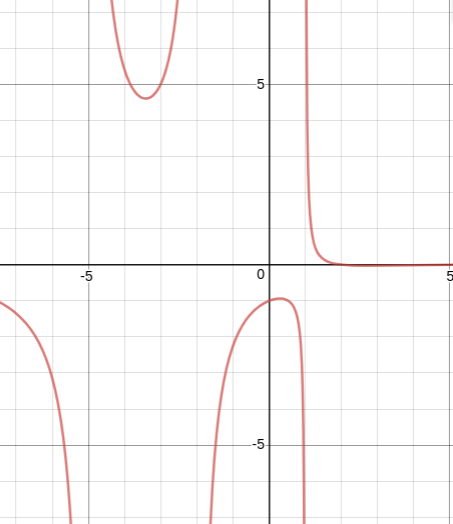
\includegraphics[width=0.5\textwidth]{../Figures/identifyGraphOfRationalFunctionC.png}
\end{center}
\begin{enumerate}[label=\Alph*.]
\item \( f(x)=\frac{x^{3} -6 x^{2} -16 x + 96}{x^{3} -31 x -30} \)
\item \( f(x)=\frac{x^{3} +6 x^{2} -16 x -96}{x^{3} -31 x + 30} \)
\item \( f(x)=\frac{x^{3} +6 x^{2} -16 x -96}{x^{3} -31 x + 30} \)
\item \( f(x)=\frac{x^{3} +6 x^{2} -16 x -96}{x^{3} -31 x -30} \)
\item \( \text{None of the above are possible equations for the graph.} \)

\end{enumerate} }
\litem{
Determine the horizontal and/or oblique asymptotes in the rational function below.\[ f(x) = \frac{12x^{3} +13 x^{2} -37 x -30}{4x^{2} -9 x -9} \]\begin{enumerate}[label=\Alph*.]
\item \( \text{Horizontal Asymptote of } y = 3.0 \text{ and Oblique Asymptote of } y = 3x + 10 \)
\item \( \text{Horizontal Asymptote at } y = 3.0 \)
\item \( \text{Horizontal Asymptote of } y = 3.0 \text{ and Oblique Asymptote of } y = 3x + 10 \)
\item \( \text{Oblique Asymptote of } y = 3x + 10. \)
\item \( \text{Horizontal Asymptote of } y = 3.0  \)

\end{enumerate} }
\litem{
Which of the following functions \textit{could} be the graph below?
\begin{center}
    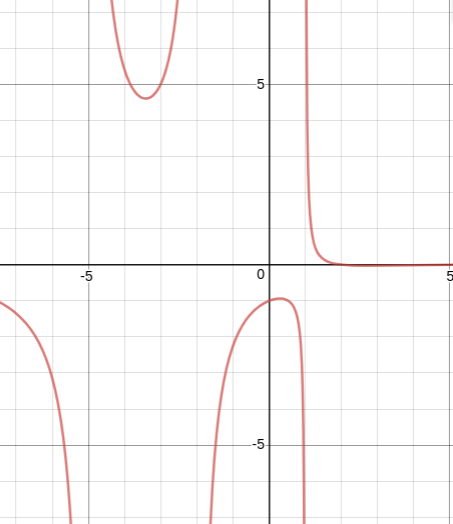
\includegraphics[width=0.5\textwidth]{../Figures/identifyGraphOfRationalFunctionCopyC.png}
\end{center}
\begin{enumerate}[label=\Alph*.]
\item \( f(x)=\frac{x^{3} +10 x^{2} +31 x + 30}{x^{3} +2 x^{2} -25 x -50} \)
\item \( f(x)=\frac{x^{3} -10 x^{2} +31 x -30}{x^{3} -2 x^{2} -25 x + 50} \)
\item \( f(x)=\frac{x^{3} + x^{2} -30 x -72}{x^{3} +2 x^{2} -25 x -50} \)
\item \( f(x)=\frac{x^{3} -10 x^{2} +31 x -30}{x^{3} -2 x^{2} -25 x + 50} \)
\item \( \text{None of the above are possible equations for the graph.} \)

\end{enumerate} }
\litem{
Determine the vertical asymptotes and holes in the rational function below.\[ f(x) = \frac{9x^{3} -48 x^{2} +73 x -30}{9x^{2} +9 x -10} \]\begin{enumerate}[label=\Alph*.]
\item \( \text{Vertical Asymptotes of } x = -1.667 \text{ and } x = 0.667 \text{ with no holes.} \)
\item \( \text{Vertical Asymptote of } x = 1.0 \text{ and hole at } x = 0.667 \)
\item \( \text{Vertical Asymptote of } x = -1.667 \text{ and hole at } x = 0.667 \)
\item \( \text{Holes at } x = -1.667 \text{ and } x = 0.667 \text{ with no vertical asymptotes.} \)
\item \( \text{Vertical Asymptotes of } x = -1.667 \text{ and } x = 1.667 \text{ with a hole at } x = 0.667 \)

\end{enumerate} }
\end{enumerate}

\end{document}